\section{Name of the Experiments}
 Design, simulate and implement Half adder, Full adder using dataflow, behavioral and structural modeling in VHDL.
 

\section{Theory}



Half adders are used to take two inputs and provide two outputs in form of Sum and Carry.
For inputs A  and B the expression is:\\
Sum = A XOR B\\
Carry = AB\\

Full adders are used to take in three inputs which include the previous Carry and then provide the output in form of Sum and Carry
For inputs A , B and Cin the expression is:\\
Sum = A XOR B XOR Cin\\
Carry = AB +BC + CA 


\section{Coding Techniques used}
\subsection{Data flow modeling}

Dataflow Modeling includes declaration of a target signal using logical events occurring on the particular signal. Dataflow Modeling is primarily expressed using signal assignment statements.

\subsection{ Behavioral modeling by using If statement}
Behavioral Modeling deals with the functionality of an entity. Here, the set of statements are executed sequentially in a specified order, mainly specified within a process statement. The process statement is itself a concurrent statement but inside it lies a set of statements which are all sequential in nature.

\subsection{Structural modeling }
Structural Modeling is the set of interconnected components. That is, it describes the structure. The visible components are instantiated in the declarative part of the architecture body while the declared components are instantiated with their respective interface ports in the statement part of the architecture body.

\section{Simulation and Results}
\subsection{Half Adder using Dataflow}
\begin{figure}[h!]
\centering
\includegraphics[width = \textwidth]{Exp1_1_Sch.PNG}
\caption{Schematic of the Half added using Dataflow modeling}
\label{figure:1}
\end{figure}



\begin{figure}[h!]
\centering
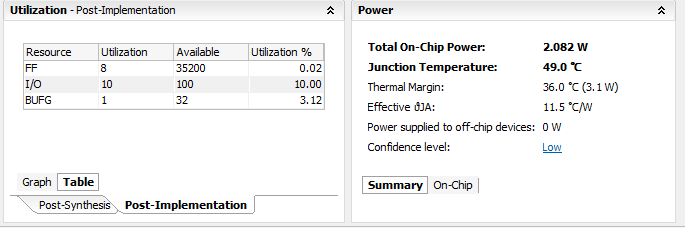
\includegraphics[width = \textwidth]{power.PNG}
\caption{Project Summary of the Half added using Dataflow modeling}
\label{figure:2}


\end{figure}


\begin{figure}[h!]
\centering
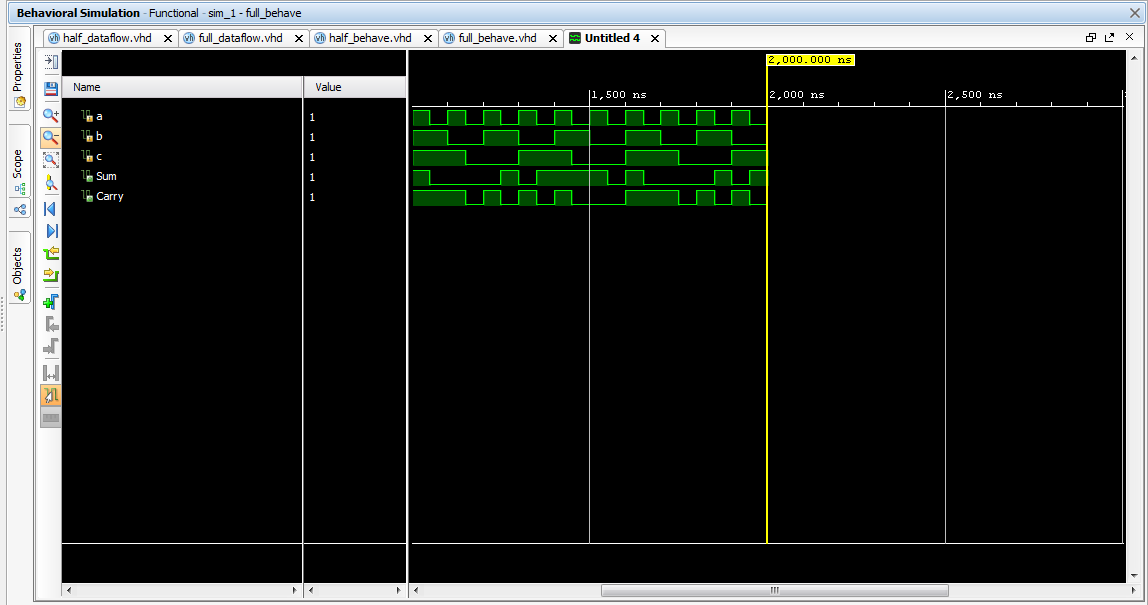
\includegraphics[width = \textwidth]{simulation.PNG}
\caption{Simulation of the Half added using Dataflow modeling}
\label{figure:3}
\end{figure}

\FloatBarrier   \clearpage

\subsection{Half Adder using Behavioural }
\begin{figure}[h!]
\centering
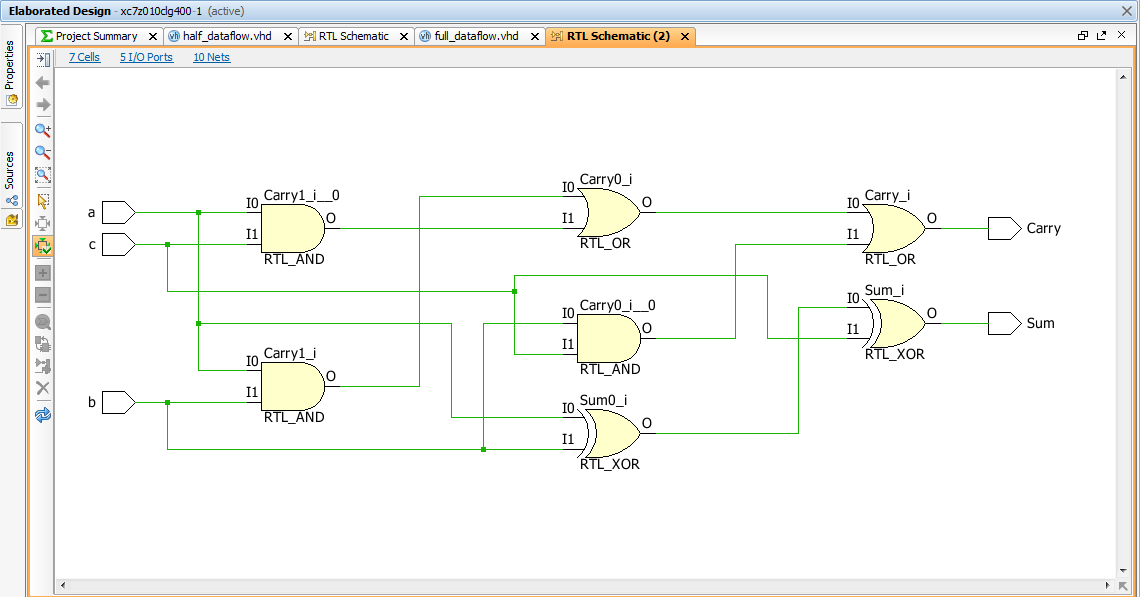
\includegraphics[width = \textwidth]{schematic.PNG}
\caption{Schematic of the Half added using Behavioural modeling}
\label{figure:1}
\end{figure}


\begin{figure}[h!]
\centering
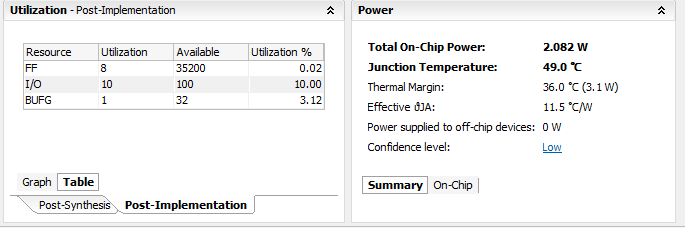
\includegraphics[width = \textwidth]{power.PNG}
\caption{Project Summary of the Half added using Behavioural modeling}
\label{figure:2}


\end{figure}


\begin{figure}[h!]
\centering
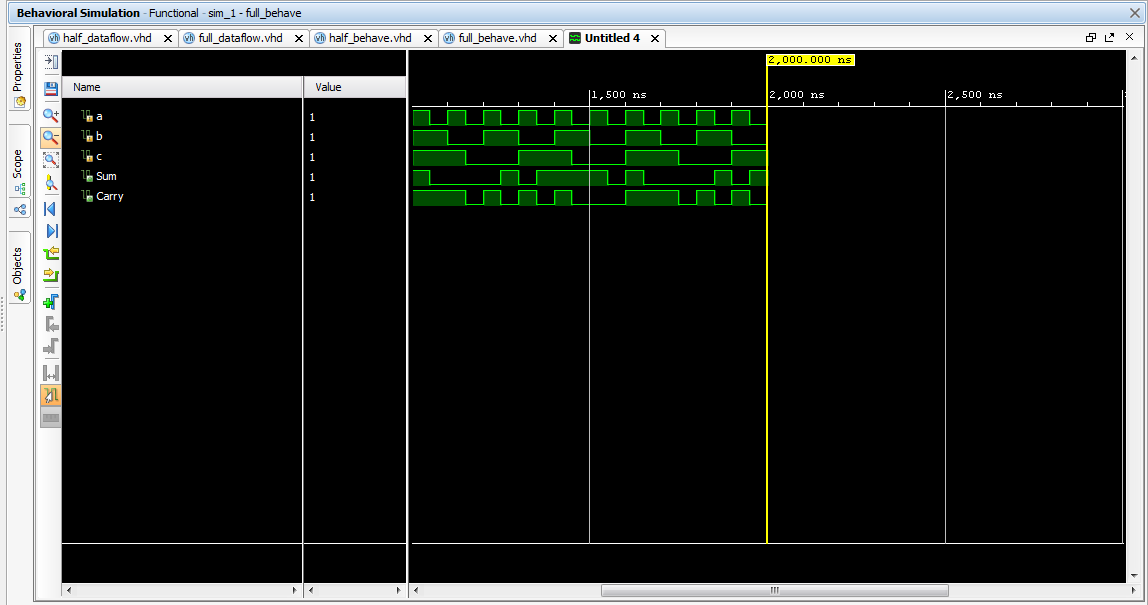
\includegraphics[width = \textwidth]{simulation.PNG}
\caption{Simulation of the Half added using Dataflow modeling}
\label{figure:3}
\end{figure}

\FloatBarrier 

\clearpage
\subsection{Full adder using half adders }
\begin{figure}[h!]
\centering
\includegraphics[width = \textwidth]{full_half_schematics.PNG}
\caption{Schematic of the Full Adder using half adder}
\label{figure:1}
\end{figure}


\begin{figure}[h!]
\centering
\includegraphics[width = \textwidth]{full_half_power.PNG}
\caption{Project Summary of the Full Adder using half adder}
\label{figure:2}


\end{figure}


\begin{figure}[h!]
\centering
\includegraphics[width = \textwidth]{full_half_simulation.PNG}
\caption{Simulation of the Full Adder using half adder}
\label{figure:3}
\end{figure}


\FloatBarrier   \clearpage

\subsection{Full adder using Behavioural modeling }
\begin{figure}[h!]
\centering
\includegraphics[width = \textwidth]{fullB_schematic.PNG}
\caption{Schematic of the Full Adder using Behavioural modeling}
\label{figure:1}
\end{figure}



\begin{figure}[h!]
\centering
\includegraphics[width = \textwidth]{fullB_power.PNG}
\caption{Project Summary of the Full Adder using Behavioural modeling}
\label{figure:2}


\end{figure}


\begin{figure}[h!]
\centering
\includegraphics[width = \textwidth]{fullB_simulation.PNG}
\caption{Simulation of the Full Adder using Behavioural modeling}
\label{figure:3}
\end{figure}


\FloatBarrier   \clearpage

\subsection{Full adder using Data Flow Modeling }
\begin{figure}[h!]
\centering
\includegraphics[width = \textwidth]{fullD_schematic.PNG}
\caption{Schematic of the Full Adder using Data flow modeling}
\label{figure:1}
\end{figure}



\begin{figure}[h!]
\centering
\includegraphics[width = \textwidth]{fullD_power.PNG}
\caption{Project Summary of the Full Adder using Data flow modeling}
\label{figure:2}


\end{figure}


\begin{figure}[h!]
\centering
\includegraphics[width = \textwidth]{fullD_simulation.PNG}
\caption{Simulation of the Full Adder using Data Flow modeling}
\label{figure:3}
\end{figure}


\FloatBarrier   \clearpage

\section{Summary}
Tabular comparison of all the codes in terms of area and power usage. 

\begin{table}[h!]
\centering
\begin{tabular}{|c|c|c|}
\hline
\textbf{Name of the Entity} & \textbf{No. of LUT used} & \textbf{Total On chip Power}\\
\hline
Half Adder using Dataflow & 1 & 0.771W \\ \hline

Half Adder using Behavioural & 1 & 0.771W \\ \hline


Full Adder using Half Adder & 1 & 1.013W \\ \hline

Full Adder using Dataflow & 1 & 1.014W \\ \hline

Full Adder using Behavioural & 1 & 1.013W \\ \hline

\end{tabular}
\caption{comparision of Area and power requirements for different kinds of adders.}
\label{tab:}
\end{table}







